\preamble{Gerunds}{Gerunds In English}
\chapter{Definition}
A gerund is a verb form that functions as a noun. A gerund is created by adding the suffix "-ing" to the base form of a verb. 
\\Like all nouns, gerunds can be used as subjects, objects of verbs, objects of prepositions, or complements.\\
\begin{center}  
    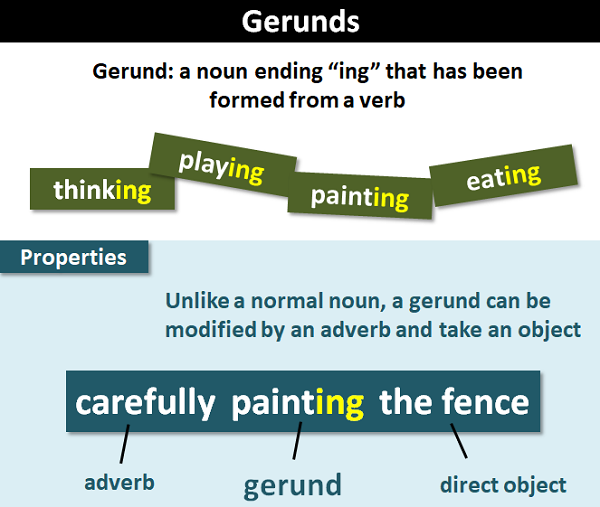
\includegraphics[scale=0.5]{project-folders/Gerunds/gerunds.png}
\end{center}

\chapter{Properties}
Unlike a normal noun, a gerund maintains some verb-like properties.\\
\textbf{For example:} 
\begin{itemize}
    \item drinking a flagon (The gerund drinking has a direct object, a flagon.)
    \item driving erratically (The gerund driving is modified with an adverb, erratically.)
    \item regularly visiting the hospital (The gerund visiting is modified with an adverb, regularly, and has a direct object, the hospital. )
\end{itemize}
\begin{center}
    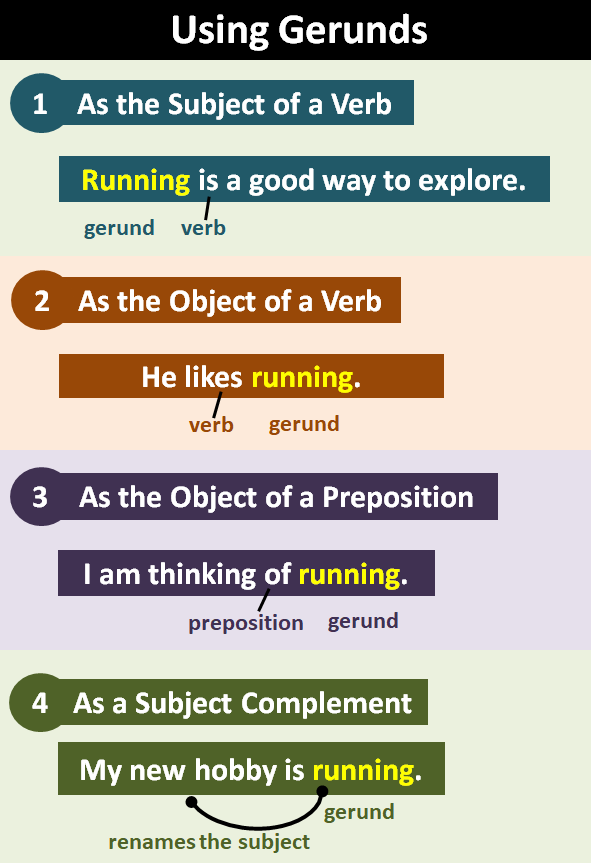
\includegraphics[scale=0.45]{project-folders/Gerunds/gerunds_use.png}
\end{center}